\subsection*{Part 2 - Extending CF's database}

\begin{enumerate}[label = {(\alph*)}]
    \item Bellow is the full ER diagram for the C.F. database.
    
    \begin{center}
        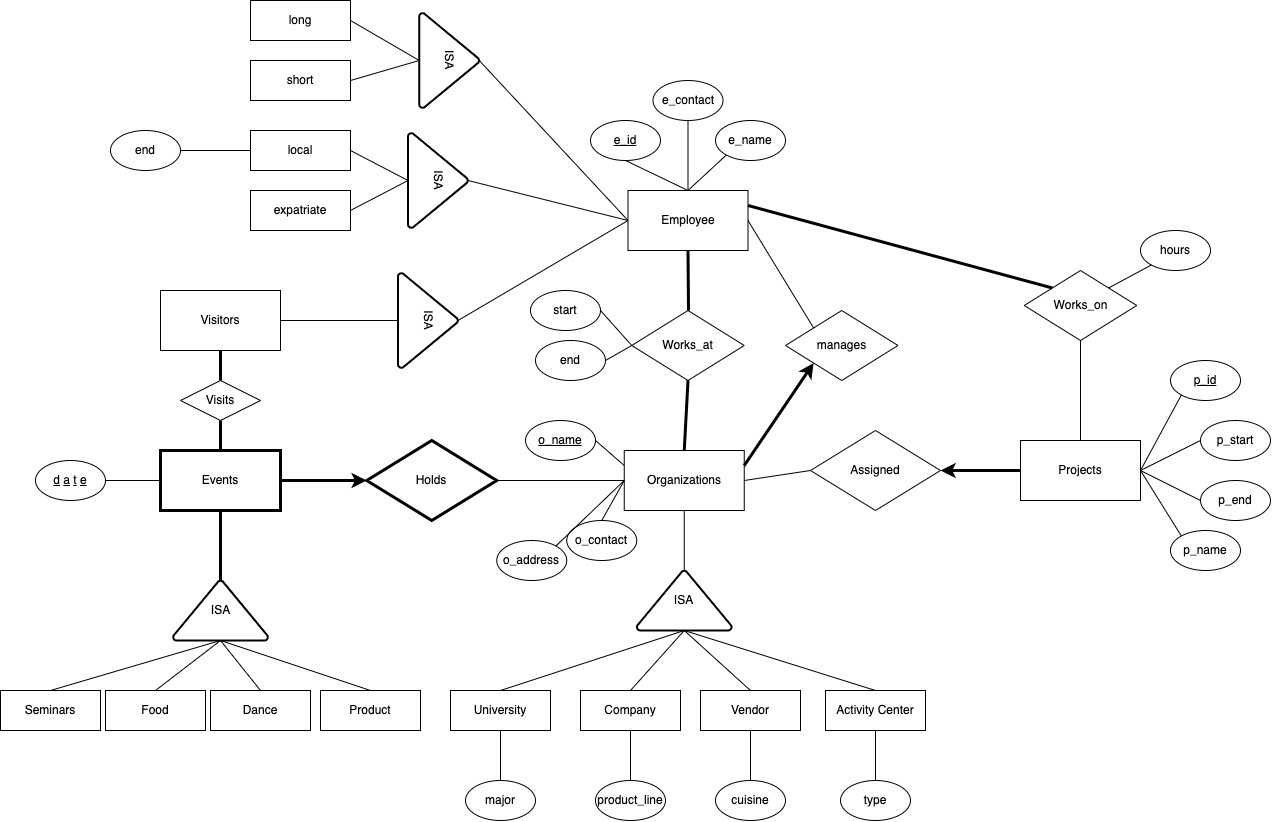
\includegraphics[width=0.9\textwidth]{img/2a.png}
    \end{center}
    \noindent We assume that all events have at least one visitor.
    
    \item 
    \begin{verbatim}
        CREATE TABLE Organizations(
            o_name: CHAR(20) NOT NULL,
            o_address: CHAR(20),
            o_contact: CHAR(20),
            PRIMARY KEY (o_name),
            UNIQUE (o_name)
            );
        
        CREATE TABLE Employees(
            e_id: CHAR(20) NOT NULL,
            e_contact: CHAR(20),
            e_name: CHAR(20),
            PRIMARY KEY (e_id),
            UNIQUE (e_id)
            );
            
        CREATE TABLE Projects(
            p_id: CHAR(20) NOT NULL,
            p_start: DATE,
            p_end: DATE
            p_name: CHAR(20),
            PRIMARY KEY (p_id),
            UNIQUE (p_id)
            );
        
        CREATE TABLE University(
            o_name: CHAR(20) NOT NULL,
            major: CHAR(20)
            PRIMARY KEY (o_name),
            FOREIGN KEY (o_name) REFERENCES Organizations 
            );
        
        CREATE TABLE Company(
            o_name: CHAR(20) NOT NULL,
            product_line: CHAR(20)
            PRIMARY KEY (o_name),
            FOREIGN KEY (o_name) REFERENCES Organizations 
            );
            
        CREATE TABLE Vendor(
            o_name: CHAR(20) NOT NULL,
            cuisine: CHAR(20)
            PRIMARY KEY (o_name),
            FOREIGN KEY (o_name) REFERENCES Organizations 
            );
            
        CREATE TABLE Activity Center(
            o_name: CHAR(20) NOT NULL,
            type: CHAR(20)
            PRIMARY KEY (o_name),
            FOREIGN KEY (o_name) REFERENCES Organizations 
            );
        
        CREATE TABLE Works_at (
            o_name: CHAR(20) NOT NULL,
            e_id: CHAR(20) NOT NULL,
            end: DATE,
            start: DATE,
            PRIMARY KEY (o_name, e_id),
            FOREIGN KEY (o_name) REFERENCES Organizations,
            FOREIGN KEY (e_id) REFERENCES Employees
            );
        
        CREATE TABLE Works_on (
            p_id: CHAR(20) NOT NULL,
            e_id: CHAR(20) NOT NULL,
            hours: TIME,
            PRIMARY KEY (p_id, e_id),
            FOREIGN KEY (p_id) REFERENCES Projects,
            FOREIGN KEY (e_id) REFERENCES Employees
            );
            
        CREATE TABLE Assigned (
            o_name: CHAR(20) NOT NULL,
            p_id: CHAR(20) NOT NULL,
            PRIMARY KEY (p_id, o_name),
            FOREIGN KEY (p_id) REFERENCES Projects,
            FOREIGN KEY (o_name) REFERENCES Organizations
            );
            
        CREATE TABLE Manages (
            o_name: CHAR(20) NOT NULL,
            e_id: CHAR(20) NOT NULL,
            PRIMARY KEY (e_id, o_name),
            FOREIGN KEY (e_id) REFERENCES Employees,
            FOREIGN KEY (o_name) REFERENCES Organizations
            );
        
        CREATE TABLE long (
            e_id: CHAR(20) NOT NULL,
            PRIMARY KEY (e_id),
            FOREIGN KEY (e_id) REFERENCES Employees
            );
            
        CREATE TABLE short (
            e_id: CHAR(20) NOT NULL,
            PRIMARY KEY (e_id),
            FOREIGN KEY (e_id) REFERENCES Employees
            );
            
        CREATE TABLE local (
            e_id: CHAR(20) NOT NULL,
            end: DATE,
            PRIMARY KEY (e_id),
            FOREIGN KEY (e_id) REFERENCES Employees
            );
            
        CREATE TABLE expatriate (
            e_id: CHAR(20) NOT NULL,
            PRIMARY KEY (e_id),
            FOREIGN KEY (e_id) REFERENCES Employees
            );
            
        CREATE TABLE Events (
            o_name: CHAR(20) NOT NULL,
            date: DATE NOT NULL,
            PRIMARY KEY (o_name, date),
            FOREIGN KEY (o_name) REFERENCES Organizations
            );
        
        CREATE TABLE Seminars (
            o_name: CHAR(20) NOT NULL,
            date: DATE NOT NULL,
            PRIMARY KEY (o_name, date),
            FOREIGN KEY (o_name, date) REFERENCES Events
            );
        
        CREATE TABLE Food (
            o_name: CHAR(20) NOT NULL,
            date: DATE NOT NULL,
            PRIMARY KEY (o_name, date),
            FOREIGN KEY (o_name, date) REFERENCES Events
            );
            
        CREATE TABLE Dance (
            o_name: CHAR(20) NOT NULL,
            date: DATE NOT NULL,
            PRIMARY KEY (o_name, date),
            FOREIGN KEY (o_name, date) REFERENCES Events
            );
            
        CREATE TABLE Product (
            o_name: CHAR(20) NOT NULL,
            date: DATE NOT NULL,
            PRIMARY KEY (o_name, date),
            FOREIGN KEY (o_name, date) REFERENCES Events
            );
            
        CREATE TABLE Visitors (
            e_id: CHAR(20) NOT NULL,
            PRIMARY KEY (e_id),
            FOREIGN KEY (e_id) REFERENCES Employees
            );
        
        CREATE TABLE Visits (
            e_id: CHAR(20) NOT NULL,
            date: DATE NOT NULL,
            o_name: CHAR(20) NOT NULL,
            PRIMARY KEY (e_id, date, o_name),
            FOREIGN KEY (e_id) REFERENCES Employees,
            FOREIGN KEY (o_name, date) REFERENCES Events
            );
    \end{verbatim}
    
\end{enumerate}